\begin{figure}[b]
\label{fig:scatdata}
\centering
	\begin{subfigure}{}
	\centering
	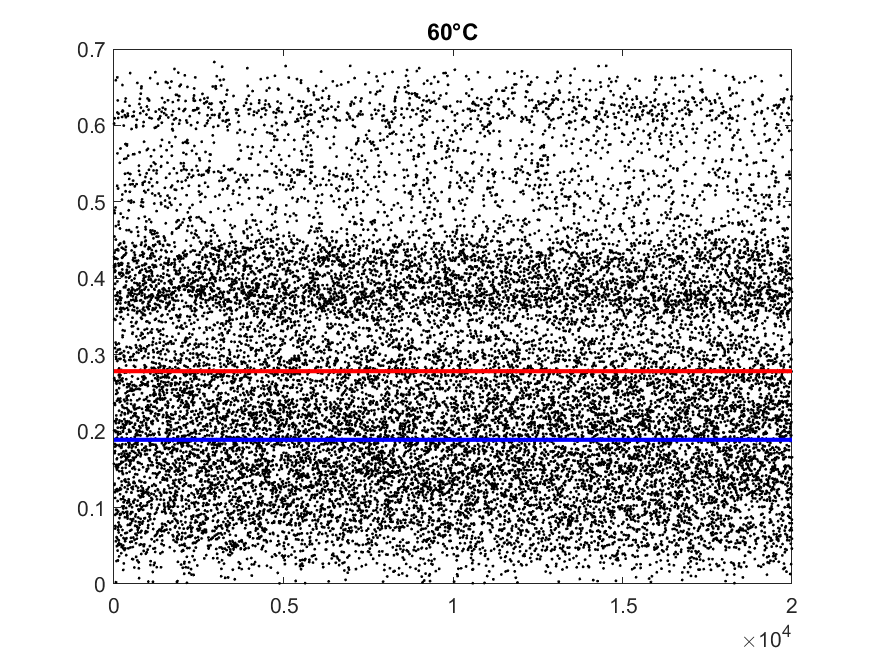
\includegraphics[width = 0.45\linewidth]{figures/histograph/scatter1.png}
	\end{subfigure}
	\begin{subfigure}{}
	\centering
	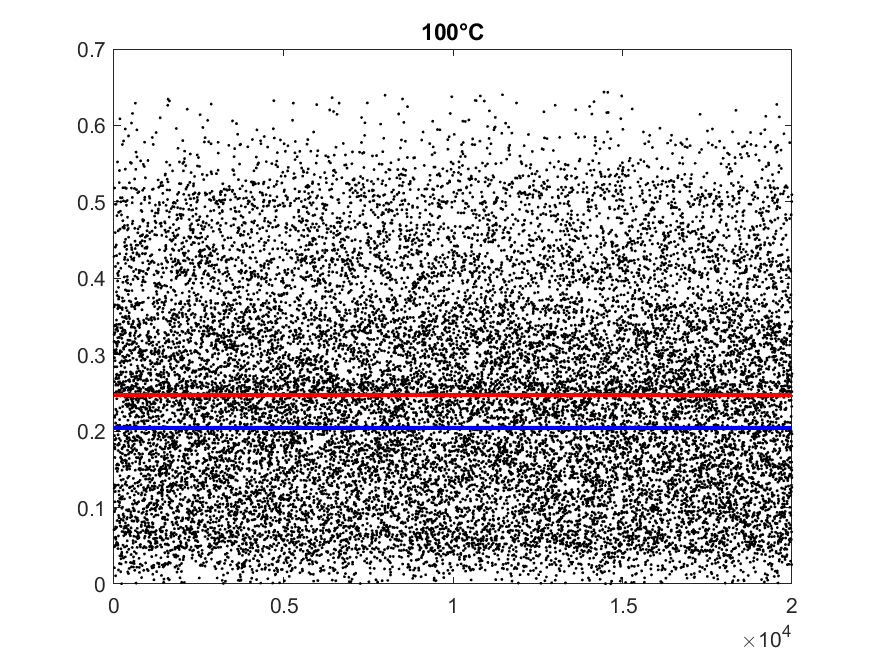
\includegraphics[width = 0.45\linewidth]{figures/histograph/scatter2.png}
	\end{subfigure}
	\begin{subfigure}{}
	\centering
	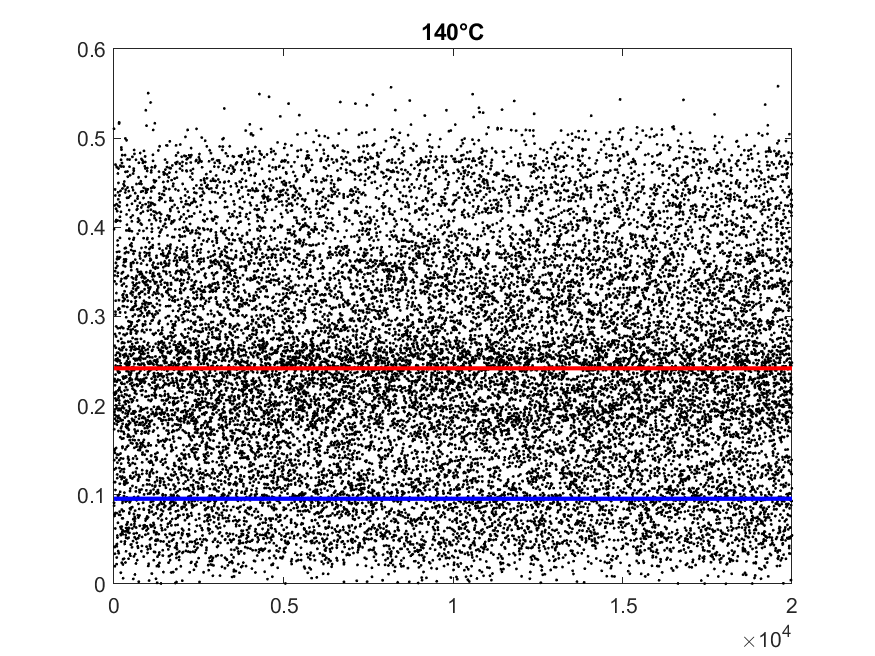
\includegraphics[width = 0.45\linewidth]{figures/histograph/scatter3.png}
	\end{subfigure}
	\begin{subfigure}{}
	\centering
	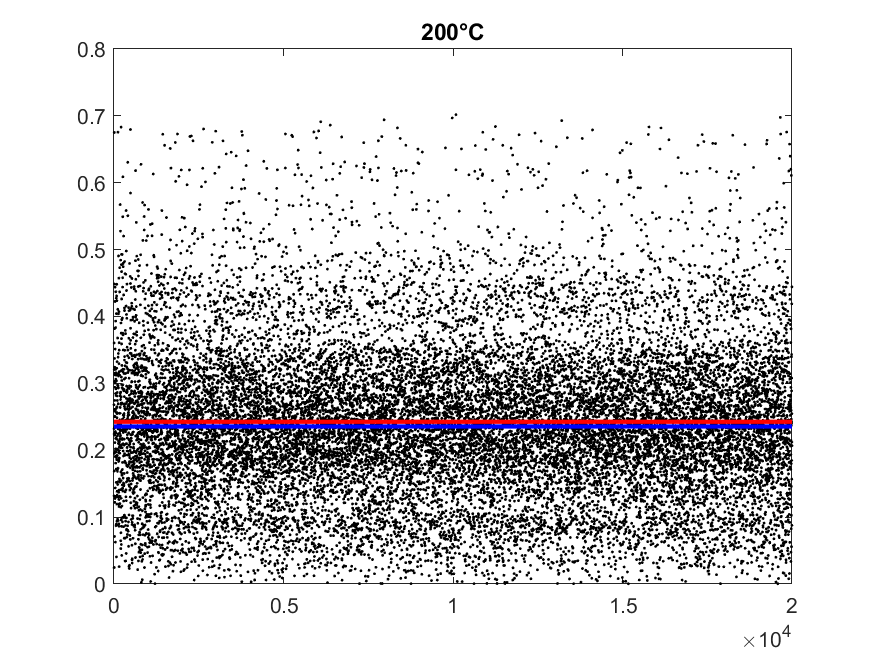
\includegraphics[width = 0.45\linewidth]{figures/histograph/scatter4.png}
	\end{subfigure}
	\begin{subfigure}{}
	\centering
	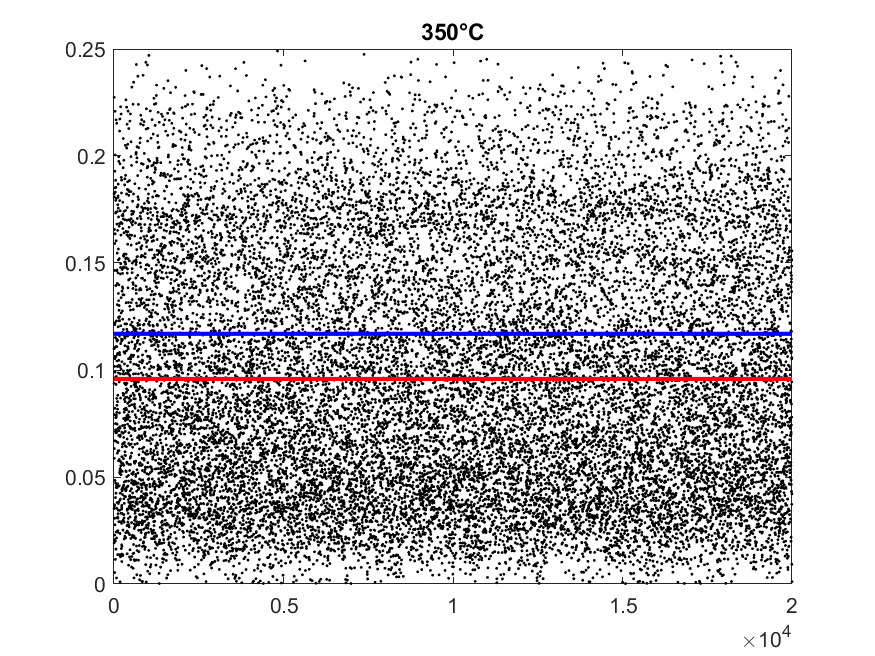
\includegraphics[width = 0.45\linewidth]{figures/histograph/scatter5.png}
	\end{subfigure}
	\begin{subfigure}{}
	\centering
	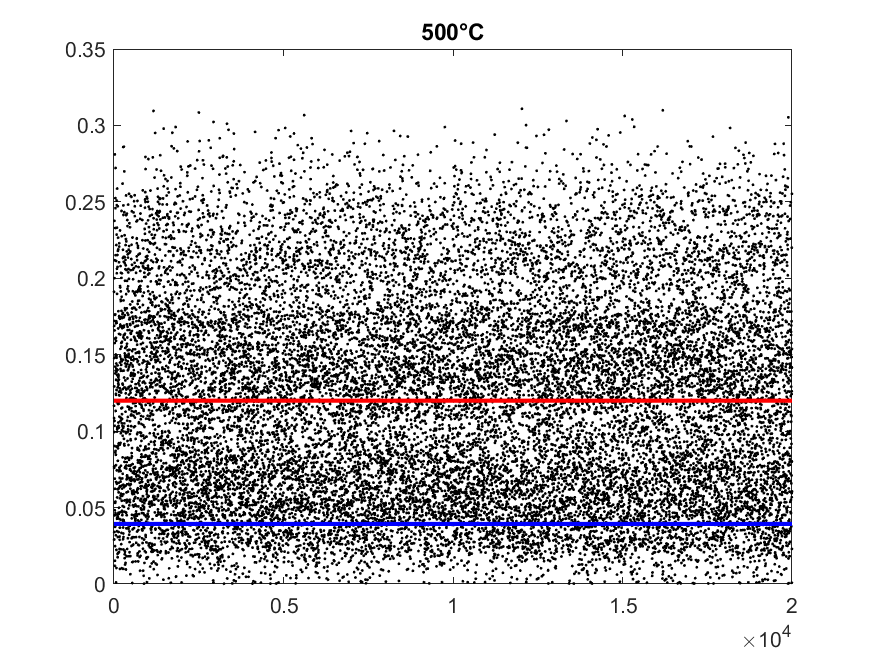
\includegraphics[width = 0.45\linewidth]{figures/histograph/scatter6.png}
	\end{subfigure}
	\begin{subfigure}{}
	\centering
	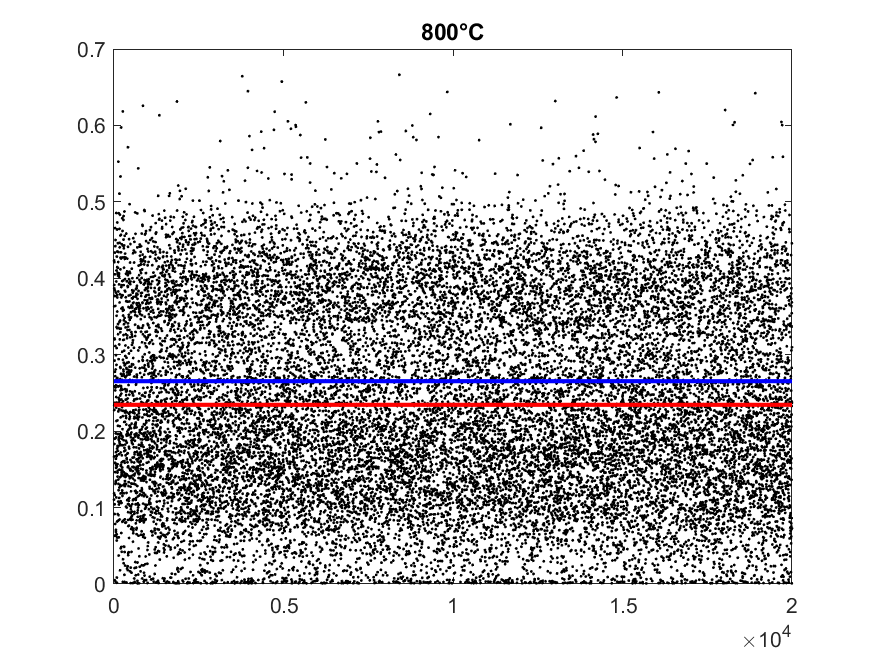
\includegraphics[width = 0.45\linewidth]{figures/histograph/scatter7.png}
	\end{subfigure}
	\begin{subfigure}{}
	\centering
	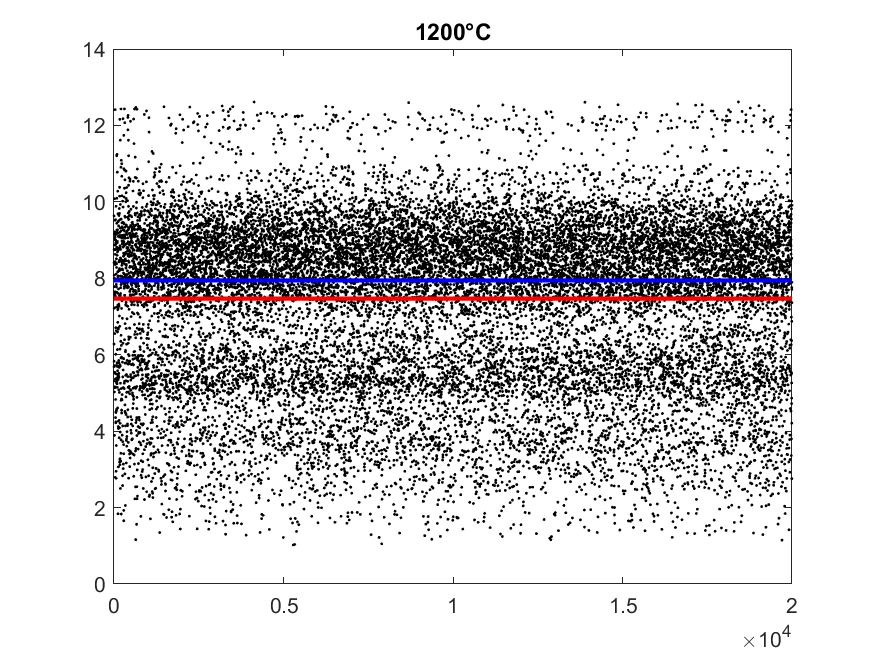
\includegraphics[width = 0.45\linewidth]{figures/histograph/scatter8.png}
	\end{subfigure}
	\centering
	\begin{subfigure}{}
	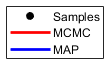
\includegraphics[width = 0.2\linewidth]{figures/histograph/scatter_legend.png}
	\end{subfigure}
	\caption{Distribution of samples at different temperatures with MCMC and MAP results indicated}
\end{figure}